\documentclass[a4paper, 10pt, fleqn]{article}

\usepackage[utf8]{inputenc}
\usepackage[T1]{fontenc}
\usepackage{textcomp}
\usepackage{lmodern}
\usepackage[ngerman]{babel}
\usepackage{tocbibind}
\usepackage{enumerate}
\usepackage{xcolor}
\usepackage{pdfpages}
\usepackage{amsmath}
\usepackage{graphicx}
\usepackage{geometry}
\usepackage{scrpage2}
\usepackage{lastpage}
\usepackage[hyphens]{url}
\usepackage{hyperref}
\usepackage{listings}
\usepackage{float}
\restylefloat{figure}
\lstset{language=[ansi]C++}

\newcommand{\code}[1]{\texttt{#1}}

\renewcommand*{\listoffigures}{%
  \begingroup
  \tocchapter
  \tocfile{\listfigurename}{lof}
  \endgroup
}

\geometry{left=3cm, top=3cm, bottom=3cm, right=2cm}

\hypersetup{
    colorlinks,
    linkcolor=black,
    citecolor=black,
    urlcolor=black
}

\pagestyle{scrheadings}
\ihead{PREN1 Gruppe 39}\ohead{Gesamtkonzept} 
\ifoot{\today} \ofoot{Seite \thepage\ von {\hypersetup{linkcolor=black}\pageref{LastPage}}}

% Einrücken zu Beginn von neuem Absatz unterdrücken
\setlength{\parindent}{0pt}

\begin{document}
% !TEX root = Dokumentation.tex
\begin{titlepage}   

\begin{center}
\textsc{\Large PREN Team 39}\\[0.5cm]

% Title
\newcommand{\HRule}{\rule{\linewidth}{0.5mm}}
\HRule \\[0.4cm]
{ \huge \bfseries GüselStar XXI}\\[0.4cm]
{ \LARGE \bfseries Gesamtkonzept}\\[0.4cm]
\HRule \\[1.5cm]

% Unterer Teil der Seite
{\large Horw, \today}

\begin{figure}[H]%Position festigen
\centering
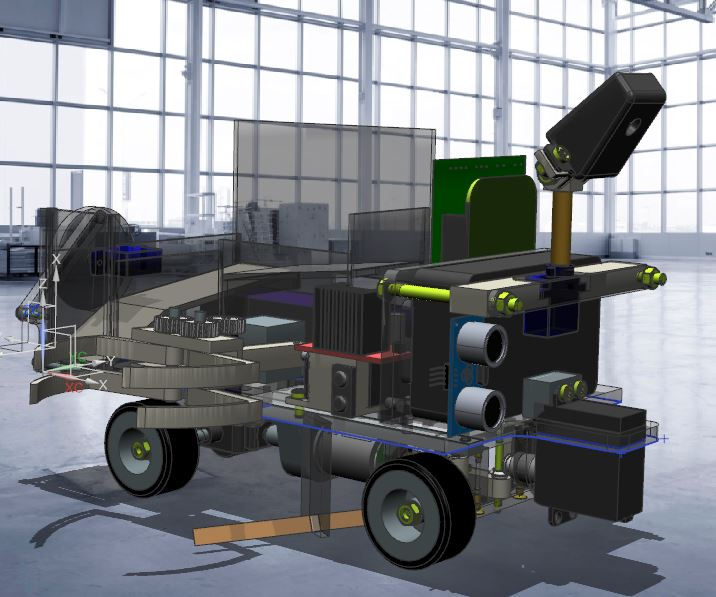
\includegraphics[width=0.7\textwidth]{03_Loesungskonzept/pictures/Tietelbild1.JPG}
\label{fig:activityRoute}
\end{figure}
% Author and supervisor
\begin{minipage}{0.4\textwidth}
\begin{flushleft} \large
\emph{Autoren:}\\
Patrizio Brantschen\\
Stefan Häfliger\\
Tobias Kreienbühl\\
Joël Meloni\\
Silvan Ritz\\
Lars Walther\\
\end{flushleft}
\end{minipage}
\hfill
\begin{minipage}{0.4\textwidth}
\begin{flushright} \large
\emph{Supervisor:} \\
Jürg Habegger
\end{flushright}
\end{minipage}
\large
\vfill
TA.BA\_PREN2.F1601 \\
Hochschule Luzern Technik \& Architektur

\end{center}

\end{titlepage}
\tableofcontents
\clearpage
\newpage
\section{Encoder}
Damit die Drehzahl des Motors ermittelt werden kann, braucht es einen Encoder. Die benötigte Hardware ist bereits auf dem Motor vorhanden. ....
\subsection{Berechnungen Encoder}
Damit man berechnen kann wie schnell das Fahrzeug fährt, muss man wissen wie viele Ticks einem cm entsprechen.
Folgende Informationen sind gegeben oder wurden gemessen:
\begin{itemize}
\item Wenn der Motor mit voller Geschwindigkeit fährt, gibt es alle 750us einen Tick
\item Der Encoder bekommt 12 High-Rise Counts pro Umdrehung (ohne Übersetzung)
\item Der Motor hat eine Übersetzung von 1:47
\item Der Raddurchmesser ist 40mm
\item Das Differential hat eine Übersetzung von 1:2
\end{itemize}

\section{Akkuüberwachung}
Damit die LiPo-Akkumulatoren nicht zerstört werden, muss sichergestellt werden das diese nicht tief entladen werden. Dies wird über das Freedomboard gelöst. Die Akkuspannung wird über einen Analog - Digitalwandler eingelesen.Wenn die Akkuspannung einen gewissen Wert unterschreiten, werden die Verbraucher an den Akkus "abgeschaltet".
\subsection{Berechungen}
Das Freedomboard kann nur Spannungen bis 3V einlesen. Daher ist ein Spannungsteiler nötig.
Für den zweiten Akku (11.1V):
\[	U_Akku/U_Frd=R1/R2\]
\[	13V/3V=4.33\]
\[	R2=10k R1=R2*4.33=43kOhm\]
Für UAkku wurde 13V gewählt, damit der AD-Wandler sicher nie 3V erreicht.\\
Für den ersten (logik) Akku (7.1V)
\[	U_Akku/U_Frd=R1/R2\]
\[	8.5V/3V=2.83\]
\[	R2=10k R1=R2*2.83=28.3kOhm\]
Für UAkku wurde 8.5V gewählt, damit der AD-Wandler sicher nie 3V erreicht.\\

\section{Encoder}
Der Encoder des Antriebsmotors wurde mit dem Motor mitgeliefert. Dies war sehr nützlich, da somit keine eigene aufwändige Lösung nötig war. Der Encoder muss mit 5V gespiesen werden. Als Ausgang hat der Encoder zwei Signale. Hier sind diese zu sehen:
\ref{fig:encoder_out}
\begin{figure}[H]%Position festigen
\centering
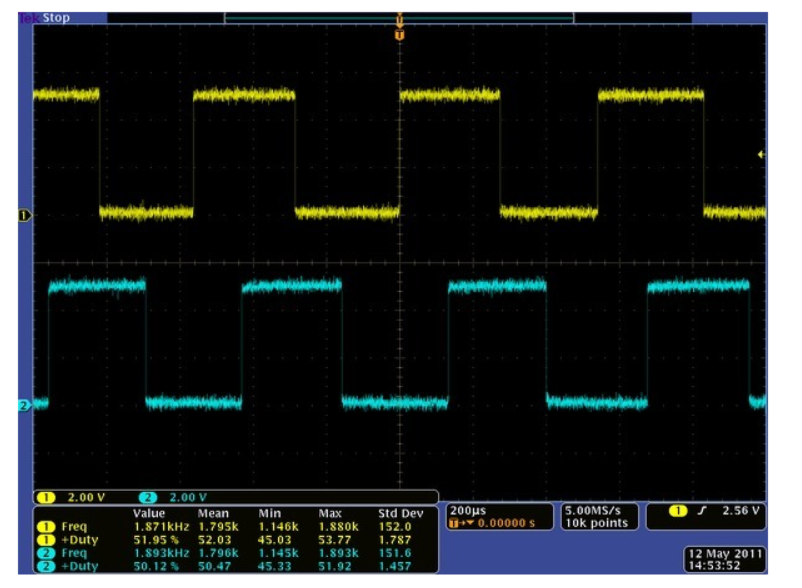
\includegraphics[width=0.6\textwidth]{Images/Encoder_Out.PNG}
\caption{Beispiels Ausgangssignal des Encoders (Quelle:pololu.com)}
\label{fig:encoder_out}
\end{figure}
Mit Hilfe dieser beiden Signalen gibt es 48 Ticks pro Umdrehung des Motors (ohne Übersetzung). Damit sind es 48Ticks/Umdrehung * 47 (Übersetzung) = 2'256 Ticks pro tatsächlicher Motorenumdrehung. Dies ergäbe eine Genauigkeit von 0.027mm/Tick bei unserem Fahrzeug. Dies ist sehr viel, darum wurde entschieden nur ein Signal auszuwerten. Damit ergibt sich eine Genauigkeit von 0.05mm/Tick. Dies ist immernoch sehr präzise.
Die Auswertung des Signales geschieht im Mikrocontrollerboard. Das Encodersiganl wird über einen Spannungsteiler auf einen Pin des Freedomboard geführt. Diese löst bei jeder Flankenänderung einen Interrupt aus. Im Interrupt wird einfach einen Zähler hochgezählt. Dieser Zähler wird alle 40ms ausgelesen und wieder auf Null gesetzt. Der ausgelesene Wert ist der Ausgangswert des Encoders. Bei voller Geschwindigkeit beträgt dieser Wert Beispielsweise 140 und bei halber Geschwindigkeit 70.
 
\section{Geschwindigkeitsregelung einstellen}
Für die Geschwindigkeitsregelung wurde ein PID-Regler verwendet. Damit die Parameter für die Geschwindigkeitsregelung richtig eingestellt sind, wurde die Schrittantwort des DC-Motors per Encoder ausgemessen. Die Schrittantwort von Null auf volle Geschwindigkeit (210RPM) sieht ungefähr so aus:
\begin{figure}[H]%Position festigen
\centering
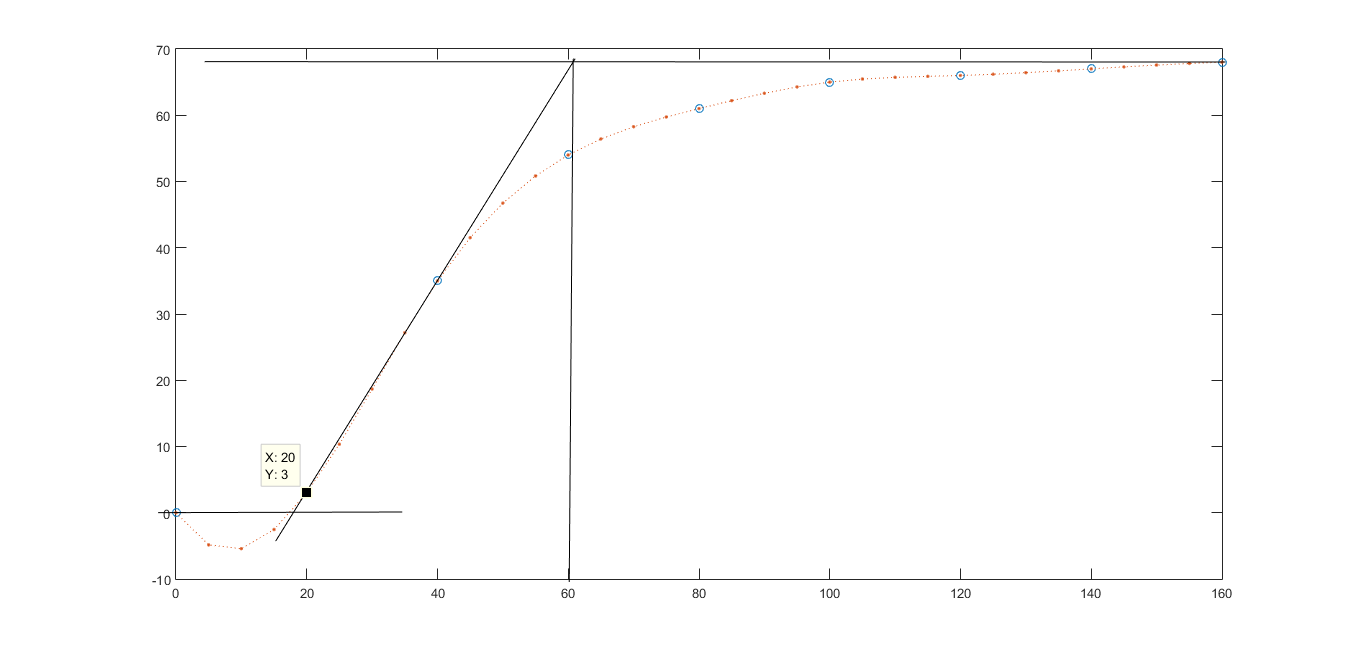
\includegraphics[width=0.9\textwidth]{Images/Sprungantwort.png}
\caption{Die Schrittantwort des DC-Motor im Matlab}
\label{fig:schrittantwort}
\end{figure}
Daraus konnten die Konstanten Tg=63ms und Tu=17ms ausgelesen werden(Einführung in die Regeltechnick S.71). Nach den Einstellregeln nach Chien-Hrones-Reswick konnten die Konstanten Tn, Tv und Kp berechnet werden(Einführung in die Regeltechnick S.215). Daraus ergaben sich die Werte Kp1=2.22, Tn=0.063, Tv=0.0085.
Diese Werte sind jedoch für kontinuierliche Regler und nicht wie in diesem Fall für diskrete Regler. Damit die Werte korrekt sind, mussten die Werte noch weiter verrechnet werden.(Einführung in die Regeltechnick S.247)
\[ T=Abtastperiodendauer=50ms\]
\[ Kp=Kp1*32=2.22*32=72\]
\[ Ki=Kp1*32*T/(2*Tn)=2.22*32*0.05/(2*0.063)=28\]
\[ Kd=Kp1*32*2*Tv/T=2.22*32*2*0.0085/0.05=5.44 =>5\]
Diese Werte sind die Regelparameter. Die Multiplikation mit 32 ergibt sich dem Grund, dass auf dem Mikrocontroller nicht mit Fließkommazahlen gerechnet wird. Somit werden die Werte bei den Parameter hochskaliert und später nach der Verrechnug mit der Regelabweichung wieder dividiert.
Diese Parameter wurden programmiert und ausgemessen. Ein Sollgeschwindigkeit von 150mm/s wurde dem Regler vorgegeben (entspricht einem Encoderwert von 108)
\begin{figure}[H]%Position festigen
\centering
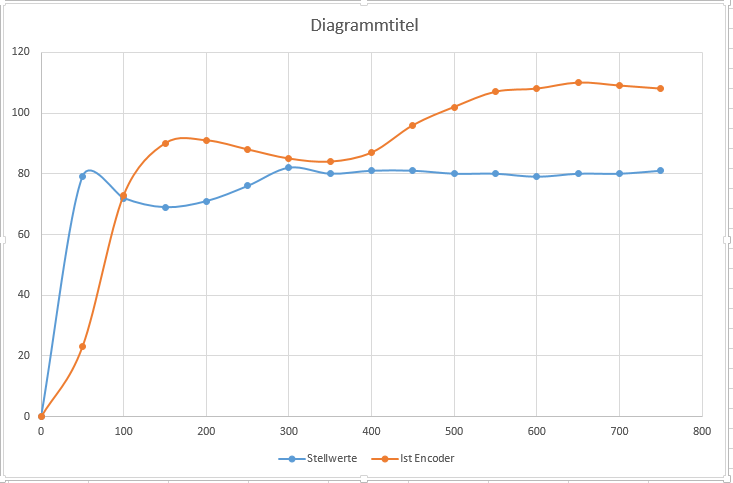
\includegraphics[width=0.9\textwidth]{Images/PID auf 150mms.PNG}
\caption{Die Istwert verglichen mit dem Stellwert}
\label{fig:IstSollwertVergleich}
\end{figure}
Hier zeigt sich, dass der Regler nicht Perfekt eingestellt ist, jedoch nach einer halben Sekunden den Sollwert erreicht hat. Dies ist für unsere Anwendung ausreichend und wird desshalb so belassen.
\section{Methodendefinitionen}
\subsection{UART-Methodenstrings}
\begin{tabular}{|l|l|l|l|l|} \hline
Aktor                 & Richtung    & String     & Übergabewert              & Bemerkungen \\\hline\hline
Ultraschall           & Frd => Rasp & Ul {}      & distance cm               & periodisch all 0.3s \\\hline
Flexsensor1 und ev 2  & Frd =>Rasp  & Fldist1 {} & distance mm               & periodisch all 0.2s \\\hline
StatusAuf             & Rasp=>Frd   & StA {}     & distance cm               & \\
                      & Frd=>Rasp   & StD        & abgeschlossen             & Wenn Aufladevorgang abgeschlossen \\\hline
StatusAb	              & Rasp=>Frd   & StA {}     & distance cm               & \\
                      & Frd=>Rasp   & StD        & abgeschlossen             & Wenn Entleeren abgeschlossen\\\hline
DC Motor	              & Rasp=>Frd   & DCDr{}{}   & cm pro sekunde	, hard/Soft & wenn nötig \\
Response DCDr new     & Frd=>Rasp   & DCDr{}{}   & cm pro sekunde            & wenn encoder say o \\\hline
Lenkungsservo         & Rasp=>Frd   & LeSer{}    & pbd                       & \\\hline
Kameraservo           & Rasp=>Frd   & CamPos{}   & einlenkungs pos           & \\\hline
Behälterentladung     & Rasp=>Frd   & Entl       & Entladungstrigger         & \\\hline
Debug Messages        & Frd=>Rasp   & DBG{}      & Debugmeldung              & \\\hline
NochDa                & Frd=>Rasp   & There      & Flag                      & periodisch all 0.5s \\
                      & Rasp=>Frd   & Ja         & Erhalten?                 & Wenn nein => DC stop \\\hline
Start                 & Rasp=>Frd   & StartFrd   &                           & Hochfahren und init \\
                      & Frd=>Rasp   & Ready      &                           & \\\hline
Stop	                  & Rasp=>Frd   & Stop       &                           & Programm beenden \\\hline
\end{tabular}
Verbesserungen/Hinzufügen:
Lenkungsservo: deg {}	Gradänderung, neu: def 	ohne Parameter =>stellt Räder auf geradeaus fahren

\end{document}
